\documentclass[man]{apa2}
\usepackage{pslatex}
\usepackage{amssymb}
\usepackage{graphicx}
\usepackage{color}
\usepackage{covington}
\usepackage[usenames,dvipsnames]{xcolor}

\title{
%Pragmatic contrast helps preschoolers learn category structure\\
%Pragmatic inferences as a route to learning category structure\\
Knowledge transmission through pragmatic inference in preschool children}

\twoauthors{Alexandra C. Horowitz}{Michael C. Frank}
\twoaffiliations{Department of Psychology, Stanford University}{Department of Psychology, Stanford University}


\abstract{Children learn many instances of cultural norms through direct instruction (e.g. ``red lights mean stop''), but not all conventional knowledge is stated explicitly.  We investigate the hypothesis that children infer generalizable information about the world pragmatically, by making inferences from speakers' descriptive word choices.  We introduced preschoolers to picture triads: an exemplar of a novel category as the base, and then two options that varied from it either by size or by a binary feature. We described the exemplar contrastively, using either a size term or another polar adjective (e.g., ``this is a [small/broken] tibu''), and asked children which of the two pictures they thought other category members looked like.  In Experiment 1, we used a supportive framing that provided an additional signal that the adjective was contrastive and found that children reliably inferred the typical category member.  In Experiment 2, children's performance was reduced when the contrastive framing was removed, but partially restored via a pre-exposure to the relevant adjective pairs. In Experiment 3, a free-response task, children spontaneously produced relevant property contrasts for both size and feature terms.  Our findings suggest that preschoolers can learn about a novel category from a single exemplar---and not just about what that category is, but also what it isn't. More generally, sensitivity to why speakers choose to describe the world the way they do may allow children to learn efficiently about the world around them. 

~\\

Keywords: pragmatics; language development; adjectives; cultural learning, social inference; production}

\shorttitle{Learning through pragmatics}
\rightheader{Learning through pragmatics}

\acknowledgements{Special thanks to the staff and families at the Bing Nursery School and the Children's Discovery Museum of San Jose and to Octavia Zahrt for assistance with Experiment 3. This work supported by a John Merck Scholars Fellowship and ONR grant N00014-13-1-0287. Earlier versions of this work were presented to the Cognitive Science Society in \citeA{horowitz2012} and \citeA{horowitz2014}.

~\\

\noindent Address all correspondence to Alexandra C. Horowitz, Stanford University, Department of Psychology, Jordan Hall, 450 Serra Mall (Bldg. 420), Stanford, CA, 94305. Phone: 650-721-9270. E-mail: \texttt{ahorowit@stanford.edu}}

\begin{document}

\maketitle                            


\section{Introduction}

Children learn some important cultural information through explicit instruction (e.g., ``put the fork on the left of the plate'') and generic statements (``forks go on the left''), but not all norms are stated directly. Sometimes information is implicit in \emph{how} a statement is made. For example, if a parent says, ``that's a salad fork,'' he is implicitly conveying that forks vary in the foods they are intended for (and that most other forks are likely used for non-salad items). More generally, the way we describe the world can reveal to a perceptive observer all sorts of biases about what we find notable, interesting, or generally worthy of comment---and such biases can in turn act as signals about our knowledge of the world. Are children able to use these implicit signals for learning? 

We test this hypothesis using a simple case study: learning to generalize novel words via minimal contrastive descriptions.  We focus on contrastive word choices, as in the above example. Contrastive word choices---the way we use labels and their modifiers---can help identify the speaker's intended referent in the current context (selecting the desired fork) but can also jointly signal generalizable knowledge (forks are associated with meal courses). In the current study, we investigate the idea that adults and children may learn generalizable knowledge via inferences about why speakers choose a particular word to convey a message. To motivate this case study, we begin by discussing two bodies of research: first, work on children's ability to learn about the world from language, and second, work on their ability to reason about the knowledge and beliefs underlying other agents' actions (both non-linguistic and linguistic). 

% This work motivates our current studies: Three experiments investigating preschoolers' generalizations about unseen category members based on speakers' word choices. 

\subsection{Learning from others' explicit statements}

Although learning from the world directly is a very powerful method for acquiring knowledge \cite{gopnik2012b}, there is no way that even the most precocious child-scientist could reconstruct an adult's knowledge from direct experience alone \cite{shafto2012,harris2012}. Instead, children's knowledge comes from a mixture of direct experiences and knowledge transmitted by others. 

Language in particular is an extremely powerful source of information about the world. From the time children begin to speak, they understand that language is used to communicate information \cite{vouloumanos2012,martin2012}. They expect speakers of the same language to use conventional names for conventional meanings \cite{clark1987, markman1988, diesendruck2005}, but learn to recognize that individual knowledge such as facts about objects may not be shared \cite{diesendruck2001}. They also show early knowledge that language can communicate about information that goes beyond the here-and-now \cite{saylor2007,ganea2007}. This early, foundational set of assumptions---that speakers will use language in consistent and communicative ways to convey (relatively) abstract knowledge---is critical in allowing children to use language to learn. 

While some language describes the particulars of the world (e.g., ``the salad fork is on the outside''), other statements provide more general information that applies across situations (``salad forks go on the outside''). Generic language---cued in a number of ways, including the use of a bare plural (``salad forks'') in the previous example---is a particularly powerful method for conveying such information \cite{leslie2008}. Children can use generic language to infer general properties quite early \cite{gelman2003}. In addition, they draw different conclusions  from generic statements than non-generic statements: They are more likely to believe that information stated generically is  conceptually and functionally central and more widely-known \cite{cimpian2009, cimpian2010, cimpian2012}. And in some contexts, generic language is not even necessary: The simple use of a label or even the use of a broader set of communicative cues---child-directed speech, direct gaze, or pointing---may signal that a speaker is presenting information that is relevant to a kind, category, or practice \cite{csibra2009, butler2012}. 
% One striking example of the role of labeling comes from a study in which \citeA{rakoczy2008} introduced 2- and 3-year-old children to a game featuring an action called ``daxing.'' Children then saw a character perform a different action and label it daxing or not.  Both age groups were more likely to protest the new action when it violated their expectations about the meaning of daxing than when it was unlabeled. By age 3 children were more likely to provide explicitly normative protests (e.g. ``It doesn't go like that'') than imperative protests (e.g. ``Use the stick''). Providing a label for the action led children to expect and enforce that the action was specific and inflexible to other interpretations.  

In fact, preschoolers find it very difficult \emph{not} to believe what they are told.  Three-year-olds can discount inconsistent evidence conveyed through physical markers (e.g. they can learn that an agent purposely places a sticker on the wrong cup, and select the opposite), but they have a much harder time discounting verbal evidence from an unreliable speaker in the same scenario. Even after telling children the \emph{wrong} location consistently, children still look for the hidden item where the speaker says \cite{jaswal2010}.  When given the option to choose between two potential informants, however, preschoolers can recognize which speaker is more accurate and prefer to trust that speaker \cite{pasquini2007}, retaining this preference even after a time delay \cite{corriveau2009}.  

% To summarize: Explicit linguistic transmission is a powerful and important source of general information about both the specific and the abstract. From an early age children are able to make use of this information, recognizing a number of different cues to the generalizability of the information in a particular statement. We next turn to work on children's ability to make inferences about the unseen causes of actions, both linguistic and non-linguistic.


\subsection{Inferences about others' actions}

% Our work is based on the idea that children make rational inferences about peopleÕs actions.  

In nearly all of the work reviewed above, a parent, teacher, or experimenter presents the relevant information explicitly, via a demonstration or explicit utterance. But a parallel line of work suggests that children and even infants are able to make inferences about the \emph{implicit} sources of both linguistic and non-linguistic actions. This literature is critical for motivating our hypothesis---that such inferences might not just inform guesses about particular agents' knowledge, abilities, preferences, or desires, but that they might also be a source of information about the world more generally. 

% We begin by discussing work on non-linguistic actions and then move on to linguistic (pragmatic) inferences.

% \subsubsection{Inferences about others' non-linguistic actions}

By their first birthday, babies appear to make inferences about the unseen goals that underly actions, even in very stripped-down displays.  For example, they look longer when a shape that previously jumped over a wall toward another shape continues on the same path when the wall is removed (an action goal) instead of moving directly toward the shape (an end-state goal; \citeNP{gergely1995}. This result is part of a broader body of work suggesting that infants expect agents to act rationally to achieve (inferred) outcomes most efficiently \cite{csibra1998, gergely2003}). In other words, very young children appear sensitive not only to agents' particular actions, but also to the presumed purpose for these actions. 

Young children also seem to be able to integrate information about constraints on knowledge and action flexibly into their inferences about goals. For example, infants can distinguish between actions that are taken intentionally (e.g. the choice of a particular ball by an agent viewing the contents of a box) versus randomly (by an agent wearing a blindfold; \cite{xu2009}.  They can also reevaluate the likelihood of particular evidence when physical constraints make it more difficult for certain items to be selected (e.g., balls that stick to velcro, \citeNP{denison2010b}).  They can even infer that the agent has a preference after observing a pattern of choices that would be unlikely to occur by random selection \cite{kushnir2010}. 

Critical for our hypothesis here, some evidence suggests that young children can also work backwards from an agent's actions to infer generalizable knowledge about objects. In an experiment by \citeA{gweon2010}, fifteen-month-olds saw a series of blue balls squeezed to make a squeaking sound and then were presented with the opportunity to generalize by squeezing a slightly different yellow ball. Depending on the evidence they saw, the children made different generalizations. If the blue balls were sampled by the experimenter from a box of blue balls (implying that they were randomly sampled by the agent), the children more likely to think that a yellow ball would also squeak. But if the children saw the blue balls picked out from a box of mostly yellow balls (where presumably the blue balls were less likely to be picked randomly, and thus were more likely to be intentionally selected for the demonstration of squeaking), they thought the yellow balls were less likely to squeak. In other words, children in this second condition made a general inference about the world (yellow balls don't squeak) based on a surprising thing that someone \emph{didn't} do (pick out yellow balls). The experiments we present below test a very related type of inference in the linguistic domain; we therefore describe some of the background for these kinds of pragmatic inference. 

% The inferences described above show a striking similarity to a quite different kind of inference: pragmatic inferences in language comprehension 

Similar to the patterns of reasoning described above, in making pragmatic inferences in language comprehension, listeners reason about the generating causes of a speaker's (linguistic) action and about the constraints on that action \cite{shafto2012}. In Grice's \citeyear{grice1975} classic example, the recommender who declares that his student has good penmanship is choosing an action that completes his goal---write a letter that is maximally informative about the student---while complying with the restrictions on his actions---be truthful, don't say anything negative. Grice famously formalized these tradeoffs in reasoning about linguistic actions as a series of maxims---be truthful, informative, relevant, and clear---and derived a number of important linguistic phenomena from their intersection. For example, on the basis of the above letter of recommendation, a reader of the letter can make the \emph{implicature} that the speaker does not believe the applicant has any other positive qualities (or else the letter writer would have mentioned them). Since Grice's initial formulation, a number of other theories have described the exact tradeoff that governs speakers' actions differently \cite{horn1984,sperber1986,clark1996,levinson2000}, even as they have preserved the basic idea of pragmatic inference as action understanding.

Are children able to make such inferences as well?  Initial work suggested that they might show deficits in this kind of pragmatic language understanding through age five or even later \cite{noveck2000,papafragou2003}: when presented with a situation where three of three horses jumped a fence, children would judge the utterance ``some of the horses jumped over the fence'' to be a felicitous description. The necessary pattern of reasoning to make the implicature in this case would be that if the speaker said ``some,'' she probably couldn't have truthfully uttered the stronger term ``all.'' A more recent body of work suggests that these deficits are specific to particular linguistic phenomena---in particular, scalar implicatures using quantifiers like ``some'' and ``all'' \cite{barner2011,katsos2011}. 

One interpretation of failures in scalar implicature tasks is that children have trouble holding in mind and contrasting the alternative statements ``some'' and ``all.'' This \emph{alternatives hypothesis} makes a number of predictions that have now been tested. First, children have difficulties with even non-pragmatic interpretations that require considering these alternatives (e.g., reasoning about what ``only some'' means; \citeNP{barner2011}). Second, exposure to alternatives increases levels of implicature \cite{skordos2014}. Third, in contexts where alternative meanings are more explicit (e.g. pictured as alternatives in a forced-choice), children perform better \cite{miller2005,stiller2014}. Thus, children appear to be more pragmatically-sophisticated than some accounts have given them credit for. We appeal to the alternatives hypothesis below in describing the developmental pattern we observe in our experiments. 

\subsection{Our current study}

Given that children are able to make a number of sophisticated inferences about the basis for both actions, we ask whether pragmatic inferences can provide a method for the transmission of information. In particular, we investigate preschoolers' ability to infer information about a general class from the specific word choice that a speaker makes in a description. For example, labeling a novel item as a ``tall blicket'' gives information not only that this item is a tall blicket, but it also suggests that height is a relevant variable property to blickets, and that other blickets may be short. 

We focus on adjectives as a case study.  Because adjectives are optional modifiers, they can be included in an utterance to draw contrasts between an intended referent and other unintended alternatives. 
% Therefore, working backwards, if the listener does not know what the unintended alternatives are, the inclusion of an adjective could convey important information about contrasts that are relevant for a particular category or comparison. In this way, an optional modifier could provide important general information about what a specific case is being contrasted with.
Children show evidence of making contrastive use of prenominal adjectives (e.g. ``red car'') in their real-time language comprehension by age 3 \cite{fernald2010}, and in more complex referential communication task by kindergarten \cite{nadig2002}. Work to date has focused on how adjectives are used in context, however.  In contrast, here we examine a novel question, asking how adjective use can help listeners infer \emph{what the context is}.  In other words, we ask whether children can infer that a contrastive description conveys not only information about the referent, but also information about the properties of other category members.

In the three experiments below, we test this hypothesis. In Experiment 1, we found that with a supportive framing, preschoolers made robust contrast inferences.  In Experiment 2, performance decreased in a more stripped down version of the task with reduced cues to contrast, but was somewhat increased by pre-exposure to the appropriate alternative set, supporting a pragmatic interpretation of this behavior. In Experiment 3, children succeeded in a more open-ended production task, suggesting that they were able to summon to mind the relevant category feature and not just select between alternatives.

\section{Experiment 1}

To investigate preschoolers' inferences about adjective use and category membership, we used a simple triad task.  We introduced children to a novel shape, followed by two similar shapes: one that differed from the first only by size, and the other that differed from the first only by a different polar feature (e.g. wet/dry).\footnote{In discussions of adjective semantics, the size adjectives we used are referred to as \emph{gradable} adjectives because their meaning is relative to the head noun \cite{kennedy2012}---a small tree is nevertheless bigger than a large mouse. In contrast, our alternative features were non-gradable---a wet sock is likely to be as wet as a wet dog. For convenience here and below, we refer to this distinction as ``size'' vs. ``feature.''} We described the first shape contrastively using either a size or feature adjective, and asked children to generalize what they thought other category members looked like. If children generalize the category without taking into account contrast, then they should expect other category members to \emph{match} on that property  (e.g., hearing ``small tibu'' and selecting that tibus are usually small). If they infer the category structure based on a contrastive interpretation, they should expect other category members to \emph{mismatch} (e.g., hearing ``small tibu'' and selecting that tibus are usually larger). 

% We wanted to investigate whether preschoolers are sensitive to information about the world that is pragmatically conveyed through speakers' word choices. We first investigated preschoolers' sensitivity to implied contrasts using familiar scalar properties. We reasoned that children may be more likely to infer contrast information when they are able to recognize that the adjective used is a member of an opposite pair (e.g. tall--short).

%  We designed a task in which the choice of adjective was the only informative cue to implicit referential contrast. If children use adjective information to generalize, they should identify other category members by matching this property. If they use adjective information to make inferences about implied contrasts, they should identify other category members by whether they contrast along the stated dimension. We found that young 3--year--olds were unable to systematically recognize category membership through speakers' adjective choices, but age 3.5, children showed sensitivity to implicit dimensions of contrast contained in word choice. By age 5, children made contrast inferences at similar rates to adults. 

\subsection{Methods}

\subsubsection{Participants}

We recruited a planned sample of 96 children into four age groups: 3.0--3.5 years (n=24, mean age 3;3), 3.5--4.0 years (n=24, mean age 3;9), 4.0--4.5 years (n=24, mean age 4;3), and 4.5--5.0 years (n=24, mean age 4;8).  Approximately half of the sample was recruited from the Bing Nursery School at Stanford University (n=52) and half was recruited from the Children's Discovery Museum (CDM) of San Jose (n=44); recruitment location was roughly even across age groups.
  
Children were tested individually in a quiet room at either the nursery school or the museum. At the CDM, parents accompanied children and sat either next to or behind the child, and children received a sticker and a certificate for their participation. If siblings also attended, they were provided quiet toys or activities such as coloring or reading during the testing prodecure. Parents were asked to fill out a short demographic form about their children's language background. As a pre-specified selection criterion, only children who were reported to hear English at least 75\% of the time were included in the final sample.  Eight participants were excluded from analysis based on this criterion.\footnote{In our partnership with the CDM, we invite any interested visitors to participate in our studies rather than prescreening children to meet our language requirements or counterbalance all demographic factors \cite{callanan2012}. Bing Nursery School is an English language preschool, and children included in the sample were fluent speakers of English. Children from Bing Nursery School and the CDM are demographically similar in terms of language exposure, ethnic backgrounds, and parental education, as reported by parents from each location.  Both locations were mainly composed of educated middle class families.  We tested for effect of location, and found no differences.}  An additional two participants were excluded for not completing all four experimental trials. 

We also recruited a comparison group of 128 adult participants through Amazon's Mechanical Turk online crowd-sourcing service.  Participants all reported being native English speakers and residents of the United States. They were informed that the task was designed for children. Three participants were excluded for failing to complete the task.  

\subsubsection{Materials}

\begin{figure}[t]
  \begin{center} 
    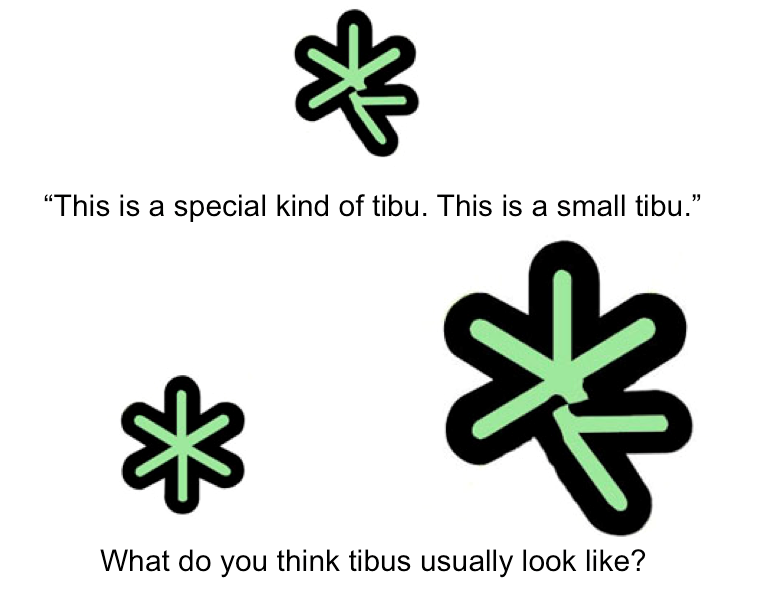
\includegraphics[width=3.5in]{figures/inanimate_demo.png} 
    \caption{\label{fig:inanimate_demo} Example of a test trial for Experiment 1a.  Participants were introduced to a base exemplar shape (top) described with either a size or feature adjective.  They were then shown two images, one that differed from the exemplar by a feature (left) and one that differed from the exemplar by size (right) and were asked to point to which picture they thought was also a member of the same category. } 
  \end{center} 
\end{figure}	

We constructed the experiment as a storybook, illustrated with colorful clipart images. Each book contained two training trials and four test trials. Each trial consisted of a novel shape (induction example) along with a pair of generalization stimuli: one that differed from the induction example only by size, and one image that differed from the exemplar only by a feature contrast (e.g., broken versus unbroken; see example in Figure \ref{fig:inanimate_demo}). Two of the four trials used size adjectives and two of the trials used feature adjectives.
% Training trials were similar but showed familiar items (e.g. chocolate milk as the induction example, with plain milk and orange juice as the generalization stimuli).  
Size terms were \emph{small} (vs. big), \emph{long} (vs. short), \emph{tall} (vs. short), and \emph{short} (vs. long);  feature contrasts were \emph{broken} (vs. unbroken), \emph{pointy} (vs. smooth), \emph{dirty} (vs. clean), and \emph{wet} (vs. dry).  To ensure that children were familiar with the words we used, we included a posttest of two-alternative displays.  Children were able to recognize all of the contrasts used in our task, with 90\% for 3--3.5 year-olds, 95\% for 3.5--4.0 year-olds, 96\% for 4.0--4.5 year-olds, and 98\% for 4.5--5.0 year-olds.  

\subsubsection{Procedure}

The experimenter read the storybook with children individually in a quiet room at either Bing Nursery School of the San Jose Children's Discovery Museum.  At the museum, parents accompanied children and sat either next to or behind the child.  Siblings were sometimes also present, and were offered quiet activities such as coloring or reading. 

To begin the book, children were introduced to a character named Allen the Alien who was visiting planet Earth.  Children then participated in two training trials containing familiar items to teach Allen about some things on Earth and get children used to the study design.  Training trials featured adjectives other than those used in critical trials, and training pictures displayed only one relevant contrast choice.  For example, children were shown a picture of chocolate milk followed by two pictures, one of plain milk and one of orange juice.  Children were told, ``This is a special kind of milk.  This is \emph{chocolate} milk.  What does milk usually look like?  What does most milk look like?" and prompted to point to the picture.  On the rare occasion that children answered incorrectly, the experimenter repeated the statements and encouraged children to point to the correct picture until they answered correctly.  

After the training trials, children participated in four test trials.  For each test trial, children were shown a picture of an induction example and told something about it, e.g. ``This is a special kind of tibu.  This is a small tibu.''  They were then shown two similar pictures, one that differed from the exemplar only by size (e.g., a big broken tibu) and one that differed from the exemplar only by a feature (e.g., a small fixed tibu), and were asked ``What do you think tibus usually look like?  What do you think most tibus look like?'' They were prompted to select one of non-exemplar images.  

Participants were assigned to one of two lists, counterbalanced for adjective type and picture order.  Adjectives were focused using contrastive stress. The experimenter averted her gaze while children pointed to their responses.  Responses were coded online and double-coded offline using a video recording of the testing session.  The task took about ten minutes to complete. 

The task was adapted to an online format for adult participants.  Adults viewed a single trial composed of one of the picture triads and read the same text that was spoken to children. We chose to use only a single trial for adults to avoid the possibility of task demands caused by repeating the same type of inference \cite{frank2012}. Picture type, side, and adjective were counterbalanced across participants.  Adults indicated their response using a radio button below their image selection.  Participants were paid 25 cents for completing the task, which took about two minutes. 

\subsection{Results and discussion}

\begin{figure}[t] 
  \begin{center} 
    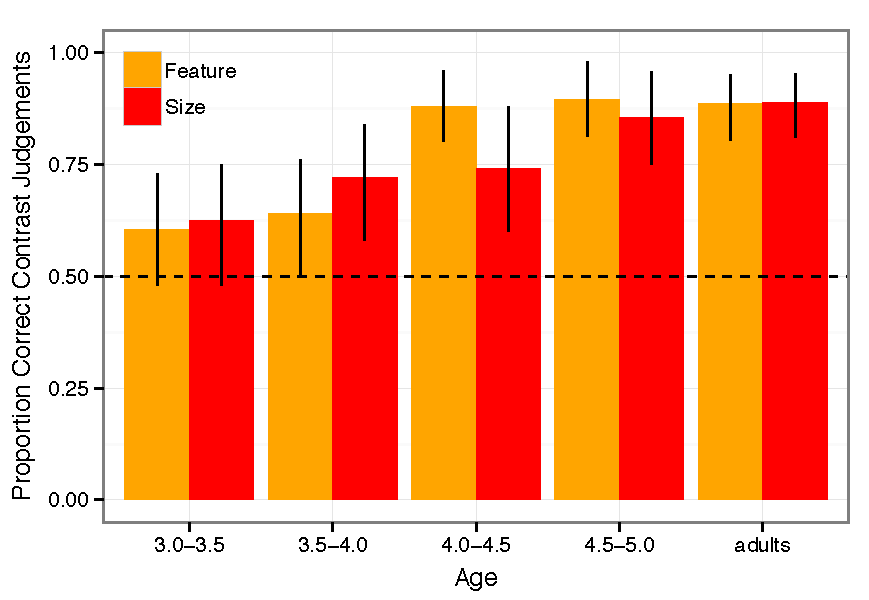
\includegraphics[width=5in]{figures/expt1_mod.pdf} 
    \caption{\label{fig:expt1_kidsAdults} Mean proportion correct for preschoolers and adults in Experiment 1. Yellow bars depict feature adjective trials and red bars depict size trials. Dashed line represents chance; error bars show 95\% confidence intervals computed by non-parametric bootstrap.}
    %95\% confidence intervals.} 
  \end{center} 
  % \vspace{-2.0ex} 
\end{figure}	

Preschoolers' ability to make correct contrast inferences increased across the age range we tested (Figure \ref{fig:expt1_kidsAdults}).\footnote{Data and analysis code can be found at \url{http://github.com/ahorowit/aliens}.} We categorized a response as correct (representing a contrast inference) if children selected the item that differed from the exemplar along the referenced dimension (e.g., they chose the short item if the exemplar was referred to as ``tall,'' but the clean item if it was described as ``dirty''). The youngest children in our sample were numerically above chance in their responding across categories ($M=.61$) but were only marginally above chance, consolidating across adjective types ($t(23) = 1.84$, $p = .08$). All other groups were above chance (all $p$s $< .01$). 

To measure differences across adjective types and age groups, we used logistic mixed effect model, predicting correct responses as the interaction of age and contrast type, with random intercept and slope (reflecting contrast type) for each participant.  Children made increasingly more correct contrast judgments with age ($\beta = 1.52$, $p < .0001$). There was no significant effect of contrast type (feature vs. size adjectives), and there was no interaction between age and contrast type, suggesting that participants across ages did not differ in their responses to different property types.  Overall, these analyses show that children demonstrate an increasing sensitivity to implicit contrast information from adjectives.  

% Rather than selecting the image that matched the named property, adults and children both selected the contrasting property.  


% Adults had no difficulty inferring contrast from adjective use in our task, and preschoolers showed a developmental increase in performance before reaching that of adults by age 5.  


\section{Experiment 2}

% In our first set of experiments, we found that adults consistently made contrast inferences from adjective use, while preschoolers gained sensitivity to how speakers mark relevant property information with age.  They may begin by appreciating that scalar opposites are paired, and that use of one term (e.g. \emph{wet}) implies contrast with its opposite (i.e. \emph{dry}). 

In Experiment 1, we provided a supportive scaffolding to help children recognize that adjectives were being used contrastively: We told them explicitly that ``this is a special kind of tibu.''  In Experiment 2, we removed this contrastive framing to test whether the older children (who succeeded handily in Experiment 1) could still make contrast inferences based on the presence of a contrasting adjective alone, a far more subtle cue. Our revised framing was ``This is a tibu. This is a small tibu.'' 

We hypothesized that this \emph{adjective only} condition would make the contrast inference substantially more difficult. Previous work on pragmatic inference has suggested that one major problem for preschool children in making inferences about contrasting terms is summoning to mind alternative terms that could have been used \cite{barner2011}. For this reason, we attempted to alleviate this burden by providing children with pre-training on the relevant contrasts of interest. In the \emph{alternatives pre-exposure} condition, we read children a book highlighting featural opposites prior to the experimental task.


\subsection{Methods}

\subsubsection{Participants}

A new sample of 96 children was recruited from Bing Nursery School.  Because of the presumed increased difficulty of this task, we recruited children from the older age groups: 4.0--4.5 years (n=48, mean age 4;4) and 4.5---5.0 years (n=48, mean age 4;9).  Half of the children in each age group (24 younger 4s and 24 older 4s) were randomly assigned to each of the conditions (\emph{Adjective Only} and \emph{Alternatives Pre-Exposure}). No children were excluded from this task. 

We also ran a new group of 128 adult participants in the \emph{Adjective Only} condition on Amazon's Mechanical Turk.  All participants were reported to be US residents and native English speakers.  They were informed that the task was designed for children.  Seven were excluded for failing to complete the task. 

\subsubsection{Materials}

\begin{figure}[t] 
  \begin{center} 
    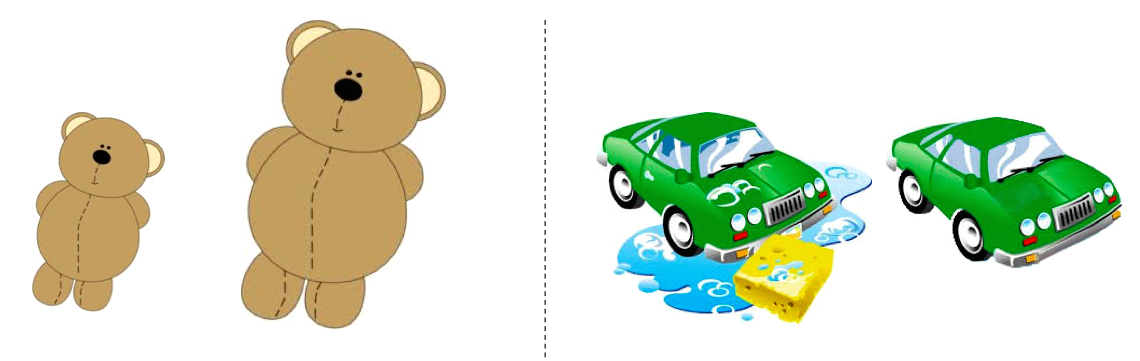
\includegraphics[width=4in]{figures/aliens_book_demo_mod.png} 
    \caption{\label{fig:book_demo} Sample images from the adjective naming book used in Experiment 3.}
  \end{center} 
\end{figure}

Stimuli were identical to Experiment 1. In the Alternatives Pre-Exposure condition, participants read a book prior to the testing procedure.  The book consisted of clip art images of familiar items depicting the size and feature contrasts portrayed in the test book. Opposites were paired so that scalar contrasts were viewed simultaneously and stated consecutively (e.g. ``Here is a small teddybear.  Here is a big teddybear.'')  Sample images are presented in Figure \ref{fig:book_demo}.


\subsubsection{Procedure}

Procedures for the experimental task were identical to Experiment 1 with the exception that the referential phrase was minimized by removing the phrase ``special kind of'' to reduce contrast cues other than the adjective.  Instead, participants heard only ``This is a [tibu]. This is a [broken tibu].''  Children in the Alternatives Pre-Exposure condition were told that they would be reading two books in the experimental session. The experimenter read the adjectives book with children, labeling each picture in a neutral way on each page (e.g. ``Here is a small teddybear. Here is a big teddybear.''). As in Experiment 1, adult participants were randomly assigned to a single test trial presented online.  

\subsection{Results and discussion}

\begin{figure}[t] 
  \begin{center} 
    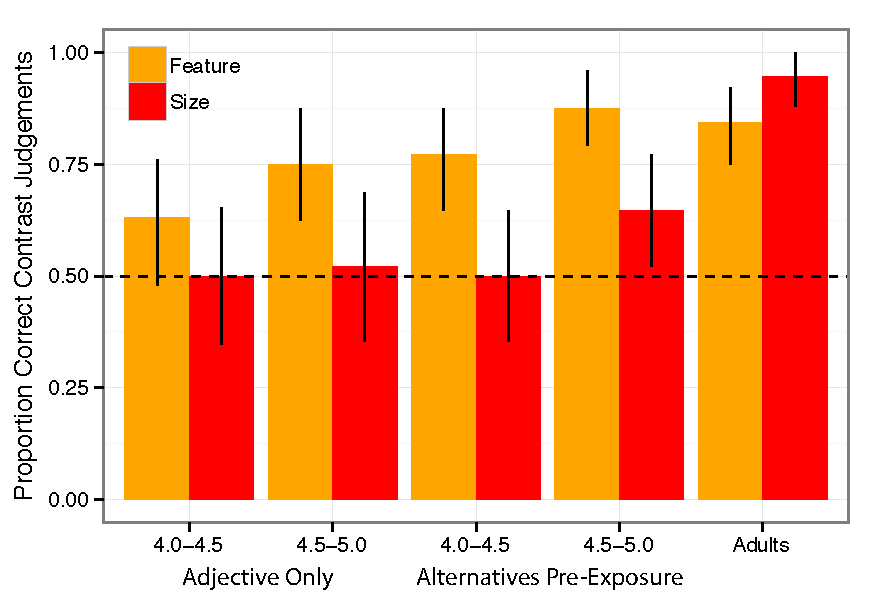
\includegraphics[width=5in]{figures/expt2_mod.pdf} 
    \caption{\label{fig:expt2_kidsAdults} Preschoolers' and adults' proportion correct performance for the \emph{Adjective Only} and \emph{Alternatives Pre-Exposure} conditions in Experiment 2. Adults did not see the pre-exposure trials. Dashed line shows chance performance; error bars show 95\% confidence intervals.}
  \end{center} 
  % \vspace{-2.0ex} 
\end{figure}

With the removal of supportive language indicating contrast, performance in Experiment 2 was substantially lower than in Experiment 1. Performance in size trials was especially low, while performance in feature trials remained higher. In the Adjective Only condition, averaging across adjective types, 4.0-year-olds were not above chance ($t(22) = 1.10$, $p = .28$), but 4.5-year-olds were ($t(23)=2.18$, $p = .04$). Breaking performance down by adjective type, on feature trials the younger 4s were marginally above chance, while the older 4s were substantially above chance ($t(22) = 1.82$, $p = .08$ and $t(23)=3.71$, $p = .001$). Both groups' performance was numerically and statistically identical to chance for size adjectives. Thus, without the contrastive language in Experiment 1, children had a substantially harder time but the oldest children could still make contrast inferences at above-chance levels for feature adjectives. 

One potential source of the asymmetry between feature and size adjectives could be due to the relatively greater contrast implied by our featural adjectives. Saying that something is ``broken'' almost always implies that it was at one time not broken. In contrast, saying something is ``small'' can imply that there are bigger others---but it can also simply reflect some sort of general, non-contrastive comment on size. If this ambiguity about the contrastiveness of the size adjectives was the source of the lowered performance in the Adjective Only condition, the Alternatives Pre-Exposure condition might increase performance for size adjectives by virtue of highlighting the contrastive use of alternative size terms. 

Congruent with this hypothesis, the alternatives pre-exposure appeared to boost performance somewhat. Children in the Alternatives Pre-Exposure condition were above chance in both conditions ($t(23) = 2.33$, $p = .03$ and $t(23) = 6.33$, $p < .0001$), aggregating across adjective types. Breaking down by adjective types, the younger 4s were above chance for feature but not size adjectives ($t(23) = 4.51$, $p = .0001$ and $t(23)=0$, $p = 1$). Older children were above chance on both ($t(23) = 8.31$, $p < .0001$ and $t(23)= 2.07$, $p = .05$). Nevertheless, no pairwise tests between the Adjective Only and Alternatives Pre-Exposure conditions reached significance. 

We again analyzed our results using a logistic mixed model. We initially fit a logistic mixed effects model specified as in Experiment 1, but found that no effects reached significance in this model, and indeed, a model that included all interactions of age, adjective type, and book type did not increase fit over a model that only included main effects ($\chi^2(4) = 2.47$, $p = .65$). This main-effects only model included a significant negative coefficient on size adjectives ($\beta = -1.08$, $p < .0001$) and marginal effects of age and book type ($\beta = 1.04$, $p = .07$ and $\beta = .50$, $p = .09$, respectively). 

In sum, Experiment 2 provides support for the hypothesis that children's judgments in Experiment 1 were strengthened by the presence of the contrastive language ``a special kind of.'' When we removed this language, performance dropped markedly, especially for size adjectives (which might not be as clearly contrastive as feature adjectives). We also saw some signs that pre-exposure to a storybook that used the target adjectives contrastively improved performance, providing additional support to the idea that it was specifically the recognition of pragmatic contrasts that led children to make the appropriate generalization. 

One possible alternative explanation for our findings is that contrast inferences were in fact not warranted by the simpler adjective framing (rather than being warranted but not being identified by children). Ruling out this explanation, the performance of adults in Experiment 2 (without supportive language) was essentially identical to that of adults in Experiment 1. Thus, we believe that the contrastive framing in Experiment 1 helped children differentially in interpreting the contrast inference implied by the use of the adjective features. 

\section{Experiment 3} 

In Experiment 3, we tested the extent of children's inferences from contrastive adjective use by examining their performance in a free-response task. One possibility in Experiments 1 and 2 was that children in fact did not infer contrast immediately from the linguistic frame and adjective, but instead recognized that the two-alternative forced choice task required a contrastive interpretation of the adjective. A free response task circumvents this issue by testing children's interpretation of the concept without asking them to choose between alternatives. For the linguistic framing in this experiment, we chose an intermediate level of support for contrast; less extreme than Experiment 1 but more supportive than Experiment 2: we told children that ``This is a plizzle. There are different kinds of plizzles. This one is a small plizzle.'' 

\subsection{Methods}

\subsubsection{Participants}

We recruited a new planned sample of 24 children (mean age 4;6) from Children's Discovery Museum of San Jose.  Only children whose parents reported that they heard English at least 75\% of the time were included in the final sample.  Two participants were excluded for using less than this amount of English, and one participant was excluded for not producing responses to the experimenter's questions.

\subsubsection{Materials}

We used a similar task design as Experiments 1 and 2, but showed children only a single picture rather than a triad.  In addition, because some of the original items depicted contrasts in which one pole was visually salient but perhaps difficult for children to name (e.g. ``broken'' vs. ``unbroken''), we modified the set of items we used.  The named size contrasts used were \emph{small} (vs. big), \emph{tall} (vs. short), \emph{long} (vs. short), and \emph{skinny} (vs. fat).  The named feature contrasts were \emph{hot} (vs. cold), \emph{dark} (vs. light), \emph{wet} (vs. dry), and \emph{open} (vs. closed).  We also ran a posttest to ensure that children were familiar with all of the properties used in the task.  Children successfully identified the contrasts 96\% of the time.

\subsubsection{Procedure}

The experimenter read the storybook with children individually in a quiet room at the CDM. As before, children were introduced to Allen the Alien and then participated in two training trials with familiar items. Unlike in  Experiments 1 and 2, children saw only a single image per trial. For example, in a training trial, children were shown a picture of a heart-shaped cookie and told, ``This is a cookie.  There are different kinds of cookies.  This one is a heart-shaped cookie.  What do other cookies look like?'' Most children answered immediately that most cookies are \emph{round} or \emph{circle}-shaped. A few children were slower to respond, and were promoted to think again what most cookies look like. If they still did not respond, they were asked what shape most cookies are.  If children provided an answer other than shape, they were encouraged to think about the description again (e.g. ``You're right, cookies can be different flavors. Did you see this one is heart-shaped?  What do most cookies look like?''). 

Following the two training trials, children participated in four test trials.  For each test trial, children were shown a picture of a single exemplar and told something about it, e.g. ``Wow, this is a plizzle. There are different kinds of plizzles. This one is a small plizzle.  What do you think other plizzles look like?'' Their verbal responses were recorded.  Two of the test trials referred to size adjectives (e.g. \emph{small}), and two of the trials referred to feature adjectives (e.g. \emph{hot}).  The order of trial items varied across two lists, each of which was counterbalanced for adjective type and picture order.  Adjectives were focused using contrastive stress. Responses were coded online and double-coded offline using a video recording of the testing session.  The task took about ten minutes to complete. 

\subsection{Results and discussion}

\begin{figure}[t] 
  \begin{center} 
    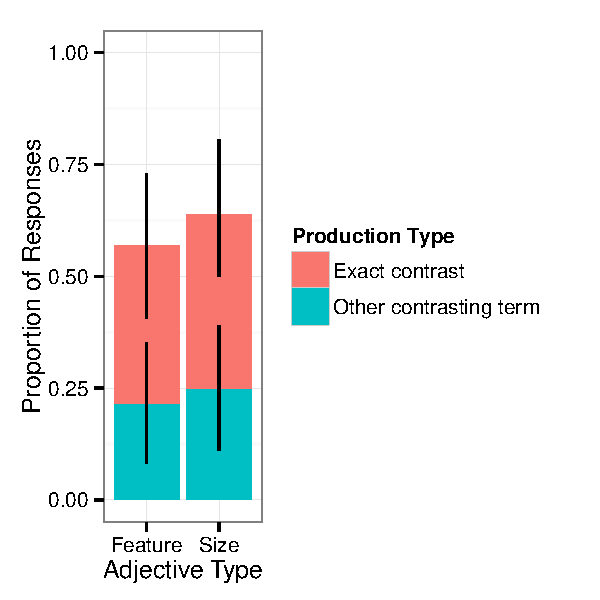
\includegraphics[width=3.5in]{figures/expt3.pdf} 
    \caption{\label{fig:freeResponse} 4-year-olds' free responses about properties of other category members upon hearing a feature adjective (left) or size adjective (right).  Productions were coded as \emph{exact contrasts} if they were opposite to the referenced description, \emph{partial contrasts} if they were related to the referenced property but not a direct contrast, or \emph{no match} if they were unrelated to the referenced modifier. }
  \end{center} 
\end{figure}

Despite the open-ended nature of the task, children gave contrastive responses more than half of the time (57\% and 64\% for feature and size).  We coded responses as either an exact contrast (e.g. hearing ``small'' and saying ``big'') or an approximate contrast to the named property (e.g. hearing ``small'' and saying a size property other than ``big'', e.g. ``tall''). Matching, non-contrastive descriptions were not included in the approximate contrast group. More than a third of productions were exact opposites (35\% for feature terms and 39\% for size terms), and another quarter were non-exact contrasts but related to the stated property information (22\% for feature terms and 25\% for size terms). There were no differences in the proportion of response scores across feature and size trials.

% Although this study provided some subtle cues about variability in this task (e.g. stating that ``There are different kinds of plizzles''), the referential expression did not particularly convey a contrastive linguistic framing the way Experiment 1 did (which stated that ``This is a special kind of...'' ).  Instead, the actual reference resembled the \emph{adjective only} framing of Experiment 2 (``This is a plizzle") and rather than pragmatically generalizing about category members (``What do most plizzles look like?'') we simply asked, ``What do other plizzles look like?''  The finding that 4-year-olds were sensitive to the informativeness of adjective use to bring to mind relevant contrast information gives further support that preschoolers are learning to use the pragmatics of word choice to infer cultural information.  Even without visually present alternatives, children still infer that adjective choice informs speakersÕ knowledge or perspective that leads them to produce the particular utterance.  


\section{General Discussion}

Our three experiments give support that children are sensitive to not just \emph{what} speakers say, but \emph{how} they say it.  We used the case study of adjectives to investigate whether children infer that speakers' modified descriptions imply knowledge about relevant dimensions of contrast. In Experiment 1, we showed that by age 3.5, preschoolers reliably made contrast inferences from size and feature adjectives with the support of a contrastive linguistic framing (``This is a special kind of tibu'').  Unlike adults, 4-year-olds in Experiment 2 had difficulty making contrast inferences when the contrast framing was removed, although their performance increased after exposure to adjective contrasts before undergoing the experimental task. Our forced-choice design may have made it especially difficult for children in Experiment 2 to reason between two plausible competitors (a property \emph{contrast} versus a property \emph{match}) from a single word cue. When these competitors were removed in our open-ended design in Experiment 3, 4-year-olds spontaneously produced relevant property contrasts the majority of the time, indicating that they can infer implied contrast information from adjective use alone, but their ability to reason backwards about pragmatic implications of word choices is still developing. Altogether, our results suggest that preschoolers appreciate adjective choice as conveying socially-relevant information about other category members. 

%
%reason about whether they should select the property \emph{contrast} conveyed in one picture or the property \emph{match} conveyed in the other picture based .  
%
%
%These findings suggest that preschoolers can infer relevant alternatives implied by word choice information, but they may rely on the support of additional cues such as a contrastive linguistic framing before spontaneously generalizing to visual competitors in our forced-choice task.  Our forced-choice task in Experiment 2 may actually be an especially challenging context for children to inter contrast because they were required to select between two plausible competitors 
%
%
%hey were required to select between one item that represented the \emph{same} property as the one stated, and one that was the \emph{contrast}.  This 
%
% In Experiment 3, we used a free response paradigm to examine childrenÕs inferences from adjective use without the constraints of the forced-choice task.  We found that, although 4-year-olds could produce any response of their liking, they spontaneously stated relevant contrast information more than half of the time.  Altogether, our results suggest preschoolers appreciate adjective choice as conveying contrast information about other category members. 

Although simple in design, our task required a fairly counterintuitive response: hearing a description and inferring its opposite. In other words, children needed to process the stated adjective and then select the picture that \emph{differed} from that description instead of the one that shared that property, even though both picture options were available. This task requires both pragmatic reasoning about how people use language, and also executive control to inhibit a matching bias to instead select the non-match.  We found that preschoolers nonetheless made these contrast inferences and robustness increased age, suggesting that they are reasoning backwards to infer contrast from speakers' word choices. Their sensitivity to the pragmatic implications of adjective use gives evidence that they are indeed processing information not just about what is stated explicitly, but also about what is culturally relevant to support such a description. 

Our studies contribute to the growing literature suggesting that children consider how and why evidence is generated to reason about the social world. By preschool age, children differentiate that random sampling conveys cues about the likelihood of distributions, while non-random sampling conveys social cues about preferences and pedagogical information \cite{xu2009, kushnir2010, butler2012}. In the domain of language, they appear to use descriptive choices to infer the implications of speakers' intended meaning to infer reference \cite<e.g.>{stiller2014}. Building on the \emph{alternatives hypothesis} that children's ability to compute implicatures relates to their recognition of linguistic alternatives \cite{barner2011}, they may need to accumulate experience with how cultural information about the world is conveyed before recognizing relevant opportunities for pragmatic inference. 


Most work to-date has focused on children's inferences about speakers' intended meaning in a referential context based on language use, and our work takes a novel approach by examining children's inferences about the state of the world that would lead a speaker to make particular production choices. While preschoolers show evidence of distinguishing generalizable knowledge from specific descriptions based on framing cues \cite{cimpian2009}, we extend these inferences to investigate children's intuitions about what world-states support contrastive descriptions.  In other words, we examine children's ability to reason about other category members not simply by generalizing the speaker's description (e.g. that hearing ``small tibu'' implies that all tibus are small), but rather by inferring property variability by pragmatic contrasts (that marking a tibu as ``small'' implies that others vary by size).  Our work suggests that children not only use modified descriptions to mark non-generic information, but they can also reason about implied alternatives specific to the adjective produced.
%Extending their understanding of rational agents and sampling \cite<e.g.>{xu2008, xu2009, gweon2010}, preschoolers may use the informativeness of word choices to consider the implied state of the world that might lead to those choices. Their sensitivity to statistical regularities in the world may help them expect that modified referents contrast with other category members along the stated property dimension (i.e. that ``big dog'' implies that dogs can vary by size).  Just as they can reason about likely sample to population of pingpong balls, language cues such as adjective use may implicitly convey cultural knowledge about the world.  In this way, word choices refer not just to references in the present (e.g. the big dog currently in sight), but also to contrasts with other possible contexts and category members (that this dog happens to be big, and others are smaller).     

%If children assume that speakers are being both rational and communicative, then they can take advantage of opportunities for inference wherever they recognize a speaker's choice to produce an utterance in one form over another.  Building on the hypothesis that children's abilities to compute implicatures relates to their ability to recognize linguistic alternatives \cite{barner2011}, children may need to accumulate experience with how cultural information about the world is conveyed before recognizing relevant opportunities for pragmatic inference. 


%Our case study of adjectives provides evidence that children are learning to process both explicit and implicitly conveyed information. Their increasing familiarity with opposite pairs leads them to robustly infer contrast with age given a supportive linguistic framing in Experiment 1 and with recency of exposure to contrasts in Experiment 2.  Without any constraints, they generated relevant alternatives on their own more than half of the time. The ability to infer culturally-implied knowledge may require both the recognition of production choices that imply alternatives and also what those particular alternatives are. 

Our work connects mechanisms of pragmatic inference, which have been well-studied in language development, with processes of social learning and generalization.  Children may need to accumulate experience with how cultural information about the world is conveyed before recognizing relevant opportunities for pragmatic inference. 
 If children assume that speakers are being both rational and communicative, then they can take advantage of opportunities for inference wherever they recognize a speaker's choice to produce an utterance in one form over another.  We show that children can figure out that naming a ``tall glorp'' implies that most glorps are shorter. The same mechanism might also allow them to infer (usefully) that the term ''cognitive scientist'' implies the existence of other types of scientists, or to infer (negatively) that ``female scientist'' implies that most scientists---at least in the mind of the speaker---are not female. Thus, pragmatic inferences of the type we study here may constitute an important mechanism of transmission for cultural knowledge.

\bibliographystyle{apacite2}
\bibliography{ADJ}

\end{document}
